\section{Discussion}


\begin{figure*}[thbp]
  \centering
  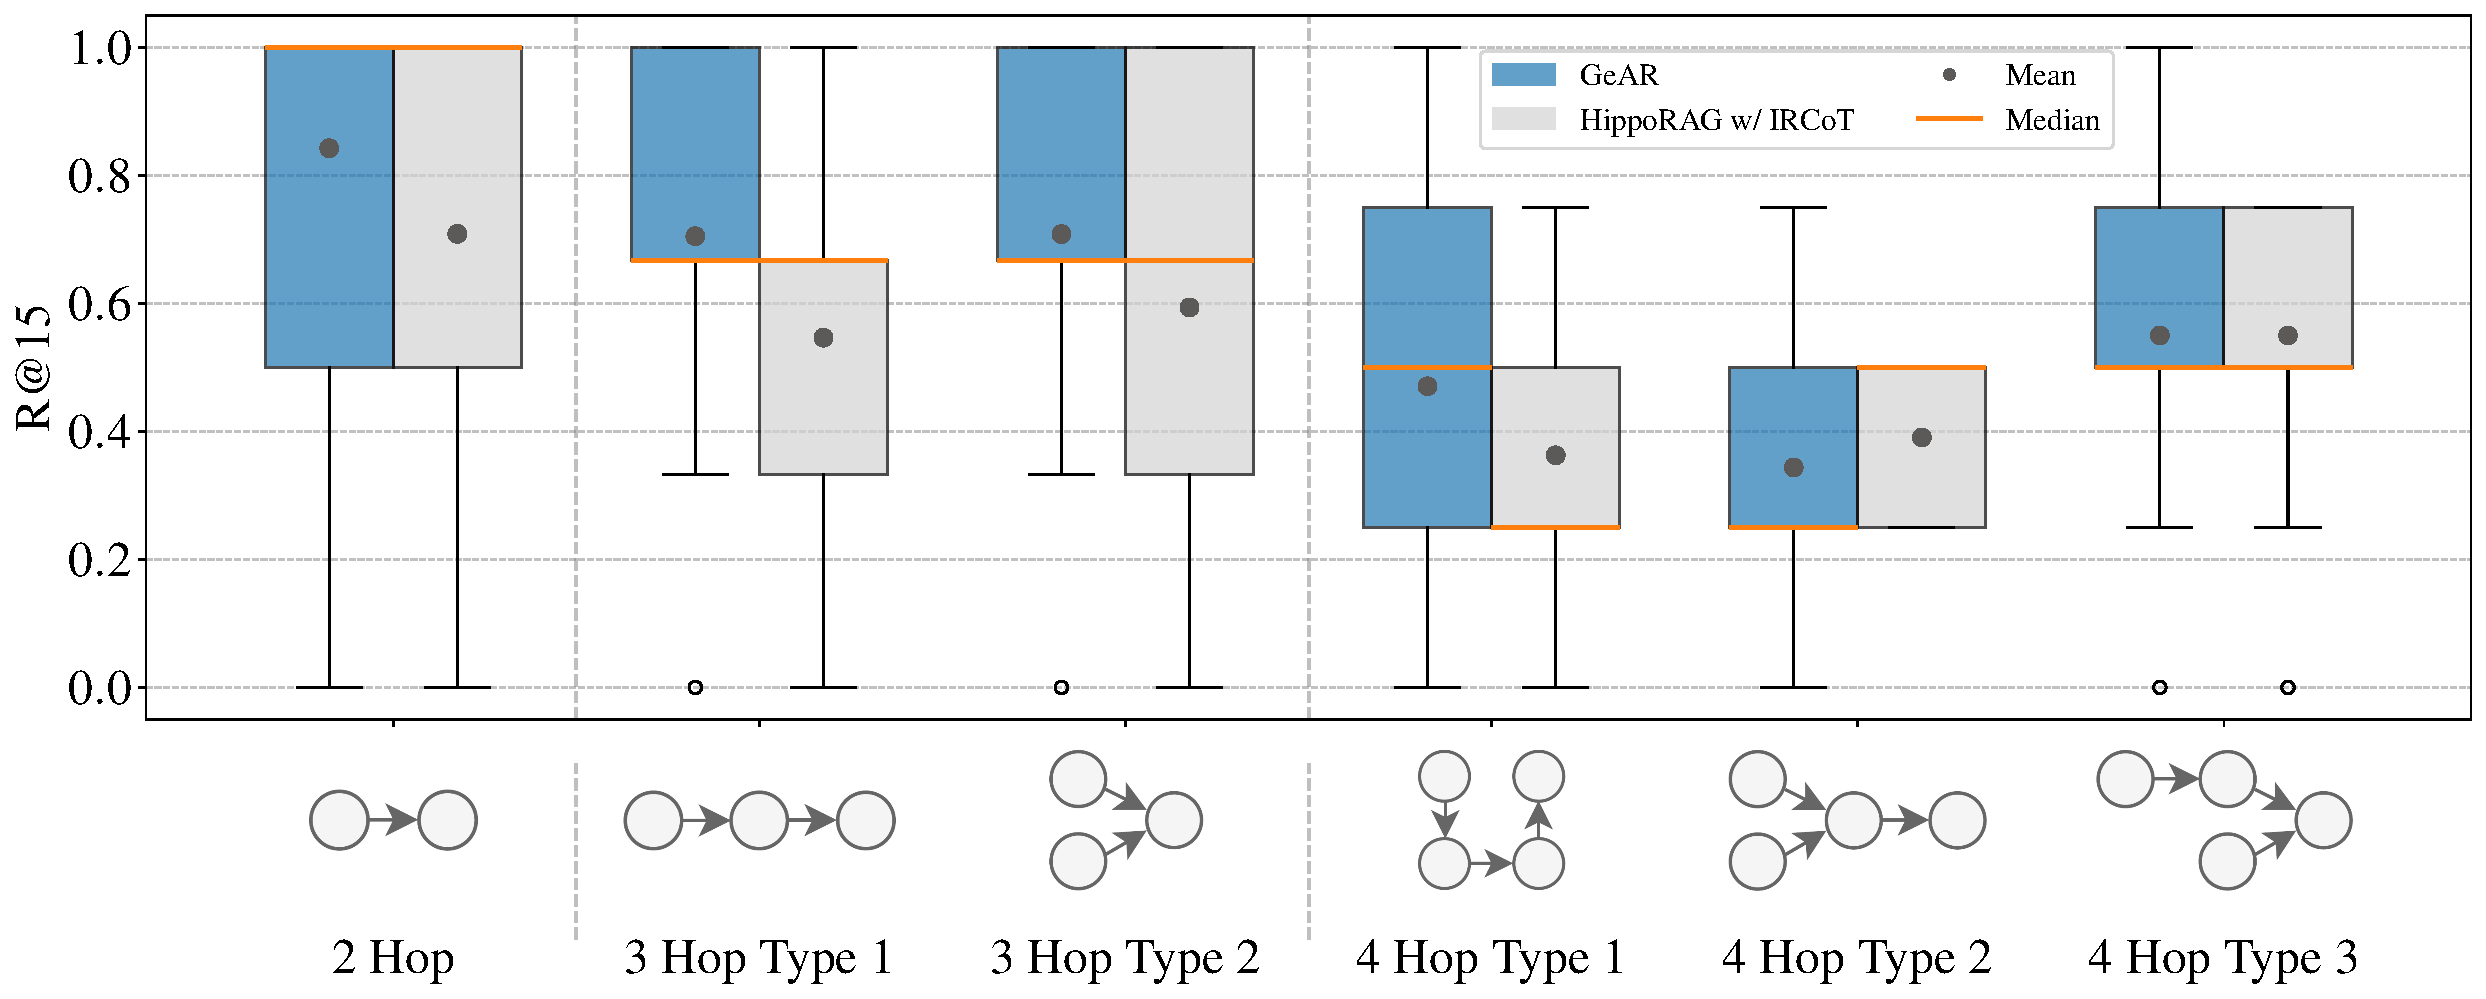
\includegraphics[width=0.92\textwidth]{figures/experiments/hoptype_vs_recall.pdf}
  \caption{Analysis of R@15 performance divided by hop types on MuSiQue. The hop categorisation follows the MuSiQue documentation. Mean recall values are indicated by grey dots for each hop type.}
  \label{fig:recall_across_hoptype}
\end{figure*}



\subsection{What makes \gear work?}
\label{subsec:what_makes_gear_work}

\paragraph{NaiveGE vs SyncGE}
As shown in Table \ref{tab:recall_main_table}, both variants of graph expansion enhance the performance of every base retriever across all datasets. The case of SyncGE is particularly interesting since without any LLM agent, it is able to surpass the retrieval performance that HippoRAG w$/$ IRCoT can achieve after several LLM iterations, on the challenging MuSiQue dataset.

\paragraph{Diverse Triple Beam Search improves performance}As shown in Table \ref{tab:diverse_beam_search}, diverse beam search consistently outperforms standard beam search across all evaluated datasets and recall ranks. By incorporating diversity weights into beam search, we align a language modelling-oriented solution with information retrieval objectives that involve satisfying multiple information needs underlying multi-hop queries~\cite{Drosou2010}.

\begin{table}[t]
\small
\centering
\begin{tabular}{l l cc}
\toprule
\textbf{Metric} & \textbf{Dataset} & \textbf{w}$\mathbf{/}$ \textbf{Diversity} & \textbf{w}$\mathbf{/}$\textbf{o Diversity} \\ 
\midrule
\multirow{3}{*}{R@5} & MuSiQue & $\mathbf{48.7}$ & $47.0$ \\
& 2Wiki & $\mathbf{72.6}$ & $68.2$ \\
& HotpotQA & $\mathbf{87.4}$ & $85.0$ \\
\midrule
\multirow{3}{*}{R@10} & MuSiQue & $\mathbf{57.7}$ & $53.9$ \\
& 2Wiki & $\mathbf{80.9}$ & $76.0$ \\
& HotpotQA & $\mathbf{93.3}$ & $92.2$ \\
\midrule
\multirow{3}{*}{R@15} & MuSiQue & $\mathbf{61.2}$ & $58.4$ \\
& 2Wiki & $\mathbf{82.4}$ & $77.4$ \\
& HotpotQA & $\mathbf{95.2}$ & $94.3$ \\
\bottomrule
\end{tabular}
\caption{Effects of beam search diversity on Hybrid + SyncGE retrieval performances across MuSiQue, 2Wiki and HotpotQA.}
\label{tab:diverse_beam_search}
\end{table}

\paragraph{\gear \textrm{\textit{mostly}} nails it the first time}

While \gear supports multiple iterations, Figure~\ref{fig:recall_across_iterations} shows that on MuSiQue, \gear can achieve strong retrieval performance within a single iteration. This differentiates it from the IRCoT-oriented setups that require at least $2$ iterations to reach their maximum performance. This can be attributed to the fact that \gear reads (Eq.~\ref{eq:proximal_read_agent}) multi-hop contexts and associates the summarised proximal triples in the gist memory with passages, establishing a synergetic behaviour between our graph retriever and the LLM. We believe this mirrors the hippocampal process of forming and resolving sparse representations, where gist memories are learnt in a one or few-shot manner \cite{Hanslmayr2016}. The performance difference between Hybrid + SyncGE and \gear at $n=1$, approximately $10\%$, indicates that the involved LLM \textit{reading} and linking processes can effectively approximate the role of hippocampus within our framework.




\subsection{Where does \gear demonstrate performance gains?}
\paragraph{\gear excels at questions of low-to-moderate complexity}

Figure \ref{fig:recall_across_hoptype} presents a detailed breakdown of retrieval performance across different hop types in MuSiQue. For 2-hop questions, while \gear and HippoRAG w$/$ IRCoT achieve similar interquartile ranges, \gear demonstrates a notably higher mean recall, indicating superior performance on low-complexity questions. This advantage becomes more pronounced with 3-hop questions, where \gear's entire interquartile range exceeds HippoRAG w$/$ IRCoT's median performance across both types of hop subdivisions. This demonstrates  \gear's enhanced capability in handling questions of moderate complexity.


\subsection{Is \gear efficient?}
\label{subsec:gear_efficient}
\paragraph{\gear requires fewer iterations}
As we observe in Figure~\ref{fig:recall_across_iterations}, \gear requires fewer iterations than the competition to reach its maximum recall performance. We attribute this to the fact that SyncGE enables \gear to bridge passages across distant reasoning hops, resulting in fewer iterations.





\paragraph{GeAR requires fewer LLM tokens}In Figure~\ref{fig:token_comparison_input_output}, we showcase that \gear can act as a more efficient alternative with respect to LLM token utilisation\footnote{Tokenisation performed using OpenAI's \texttt{tiktoken} tool.}. We observe that even for a single iteration, \gear uses fewer tokens than HippoRAG w$/$ IRCoT. In contrast to ours, this trend exacerbates for the competition as the number of iterations increases. The findings from this figure also reiterate the value of SyncGE (see Section~\ref{subsec:what_makes_gear_work}), which is able to outperform a significantly more LLM-heavy solution in MuSiQue, using almost $2.9$ million fewer tokens. Even in the case that HippoRAG w$/$ IRCoT runs for a single iteration it would require more than $0.7$ million tokens that Hybrid + SyncGE, with a substantially lower R@15 of $51.7$.

\begin{figure}[thbp]
  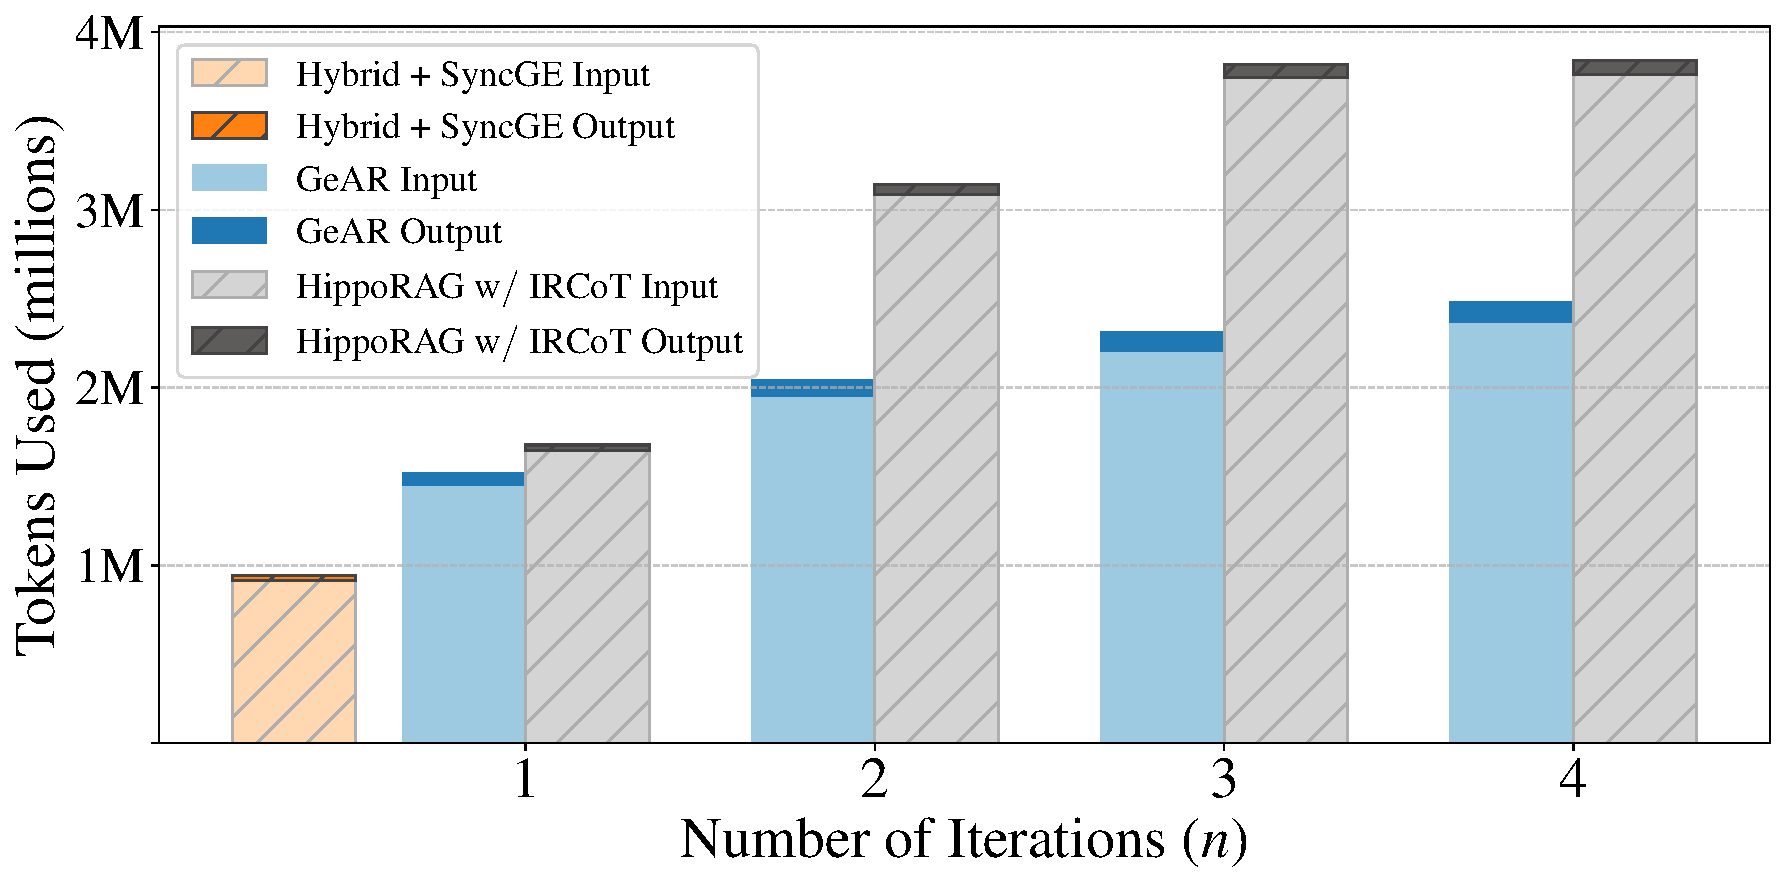
\includegraphics[width=\linewidth]{figures/experiments/tokens_vs_agent_iters_input_output.pdf}
  \caption{Progressive accumulation of input and output LLM tokens across agent iterations on MuSiQue.Token counts at each iteration build upon previous ones, resulting in monotonically increasing token counts to demonstrate the cumulative nature of multi-step approaches. Tokenisation is performed using OpenAI's `tiktoken' open-source tool. The Hybrid + SyncGE method appears only in Iteration $1$ as it is a single-step approach.}
\label{fig:token_comparison_input_output}
\end{figure}
